\setlength{\footskip}{8mm}

\chapter{RESULTS}
\label{ch:results}

\textit{In this chapter we will see the implementation of the Argumentation Framework applied to a case. The Laws, Contract and Arguments themselves are represented in Prolog, a logic programming lanuage; The Argument Processessing Unit and the Argument Generation Unit as well as the user interface are written in a hybrid of Prolog and Python, an interpreted, high-level and general-purpose programming language }

\section{Representing the Contract and Laws}

The insurance policy and the laws are represented as Prolog programs which all parties agree on.

The rules defined here are later queried to check if the contract applies or not.

\subsection{Representing the Arguments}

Each argument is represented in a separate file as a Prolog program. Each file starts with Prolog comments which are used as annotations to define the name of the argument and attack relations between arguments.

The body of the program represents how a rule is interpreted by the argument.

The programs' are structured as follows:

\begin{verbatim}
    % argument <NAME OF THIS ARGUMENT>
    % attacks <NAME OF AN ARGUMENT BEING ATTACKED>
    % attacks <NAME OF AN ARGUMENT BEING ATTACKED>
    .
    .
    .
    % attacks <NAME OF AN ARGUMENT BEING ATTACKED>
    
    <BODY OF PROGRAM>
\end{verbatim}

\subsection{Implementation of Argumentation Framework}

The Argument Generation Unit (AGU) and Argument Processing Unit (APU) \cite{dung1995} are implemented in both Python and Prolog, using the PySwip library to interface between Python and Prolog. The program goes through the argument files and generates the attack relations between the arguments using the annotations. Using these attack relations, we can find the acceptable arguments. 

Using this information we can find the grounded extensions. We then take the union of the rules as interpreted in the winning arguments and use this to query what the law means.

\subsection{Modeling claim 1 of Flota Mercante Dominicana v American Manufactureres Mutual Insurance Company}

\subsubsection{The insurance contract and contra perfortam canon}

\begin{verbatim}
% war_risk_policy.pl
    covered_by_war_risk :- war_risk, not(exemption).
    
    exemption :-
      cause_of_damage_to_ship(barratry, crew);
      cause_of_damage_to_ship(capture, government_forces);
      cause_of_damage_to_ship(seizure, government_forces);
      cause_of_damage_to_ship(arrest, government_forces);
      cause_of_damage_to_ship(restraint, government_forces);
      cause_of_damage_to_ship(detainment, government_forces);
      cause_of_damage_to_ship(preemption, government_forces);
      cause_of_damage_to_ship(confiscation, government_forces);
      cause_of_damage_to_ship(requisition, government_forces).
\end{verbatim}

\begin{verbatim}
% contra_perfortam_canon.pl
    construe_term_in_favour_of(TERM, PARTY) :-
        ambiguous(TERM),
        not(contract_written_by(PARTY)).    
\end{verbatim}

\subsubsection{The arguments}

\begin{verbatim}
    % argument p1

    cause_of_damage_to_ship(weapon_of_war, rebels).
    cause_of_damage_to_ship(weapon_of_war, americans).
\end{verbatim}
    
\begin{verbatim}
    % argument d1
    % attacks p1
    
    cause_of_damage_to_ship(barratry, crew).
    
\end{verbatim}
    
\begin{verbatim}
    % argument d2
    % attacks p1
    
    cause_of_damage_to_ship(capture, government_forces).
    
\end{verbatim}
    
\begin{verbatim}
    % argument c1
    % attacks d1
    % attacks d2
    
    cause_of_damage_to_ship(weapon_of_war, rebels).
    
\end{verbatim}
    
\begin{verbatim}
    % argument d3
    % attacks p1
    
    cause_of_damage_to_ship(weapon_of_war, rebels).
    
\end{verbatim}
    
\begin{verbatim}
    ship_damaged_after(requisition, government_forces).
    
    exemption :-  ship_damaged_after(requisition, government_forces).
    
    % argument c2
    % attacks d3
    
    cause_of_damage_to_ship(weapon_of_war, rebels).
    
    ambiguous(requisition).
    contract_written_by(defendant).
    ship_damaged_after(requisition, government_forces).
    
    exemption :-
        ship_damaged_after(requisition, government_forces),
        construe_term_in_favour_of(requisition, defendant).
 
\end{verbatim}

\subsubsection{Results}

The AGU gives us the following attack relations:

\begin{verbatim}
    attack(c1, d1).
    attack(c1, d2).
    attack(c2, d3).
    attack(d1, p1).
    attack(d2, p1).
    attack(d3, p1).
\end{verbatim}

And APU gives the following grounded extensions:

\begin{verbatim}
    [p1, c1, c2]
\end{verbatim}

This finally results in the rules from the grounded extensions:

\begin{verbatim}
% generated_rules.pl
    cause_of_damage_to_ship(weapon_of_war, rebels).
    cause_of_damage_to_ship(weapon_of_war, americans).
    
    ambiguous(requisition).
    contract_written_by(defendant).
    ship_damaged_after(requisition, government_forces).
    
    exemption :-
        ship_damaged_after(requisition, government_forces),
        construe_term_in_favour_of(requisition, defendant).
\end{verbatim}

Using these rules we can check if the war risk policy is covered.

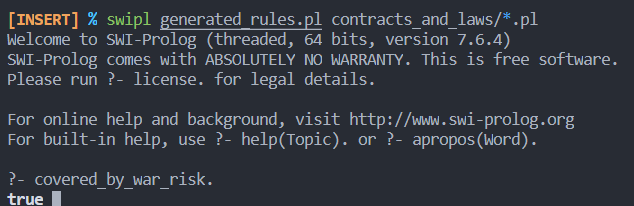
\includegraphics{figures/result.png}

\FloatBarrier